\section{RISMC approach to multi-unit modeling}
\label{sec:RISMC_MU_modeling}

This section shows in detail how the actual multi-unit model has been implemented
using RAVEN and RELAP5-3D. 

\begin{figure}
    \centering
    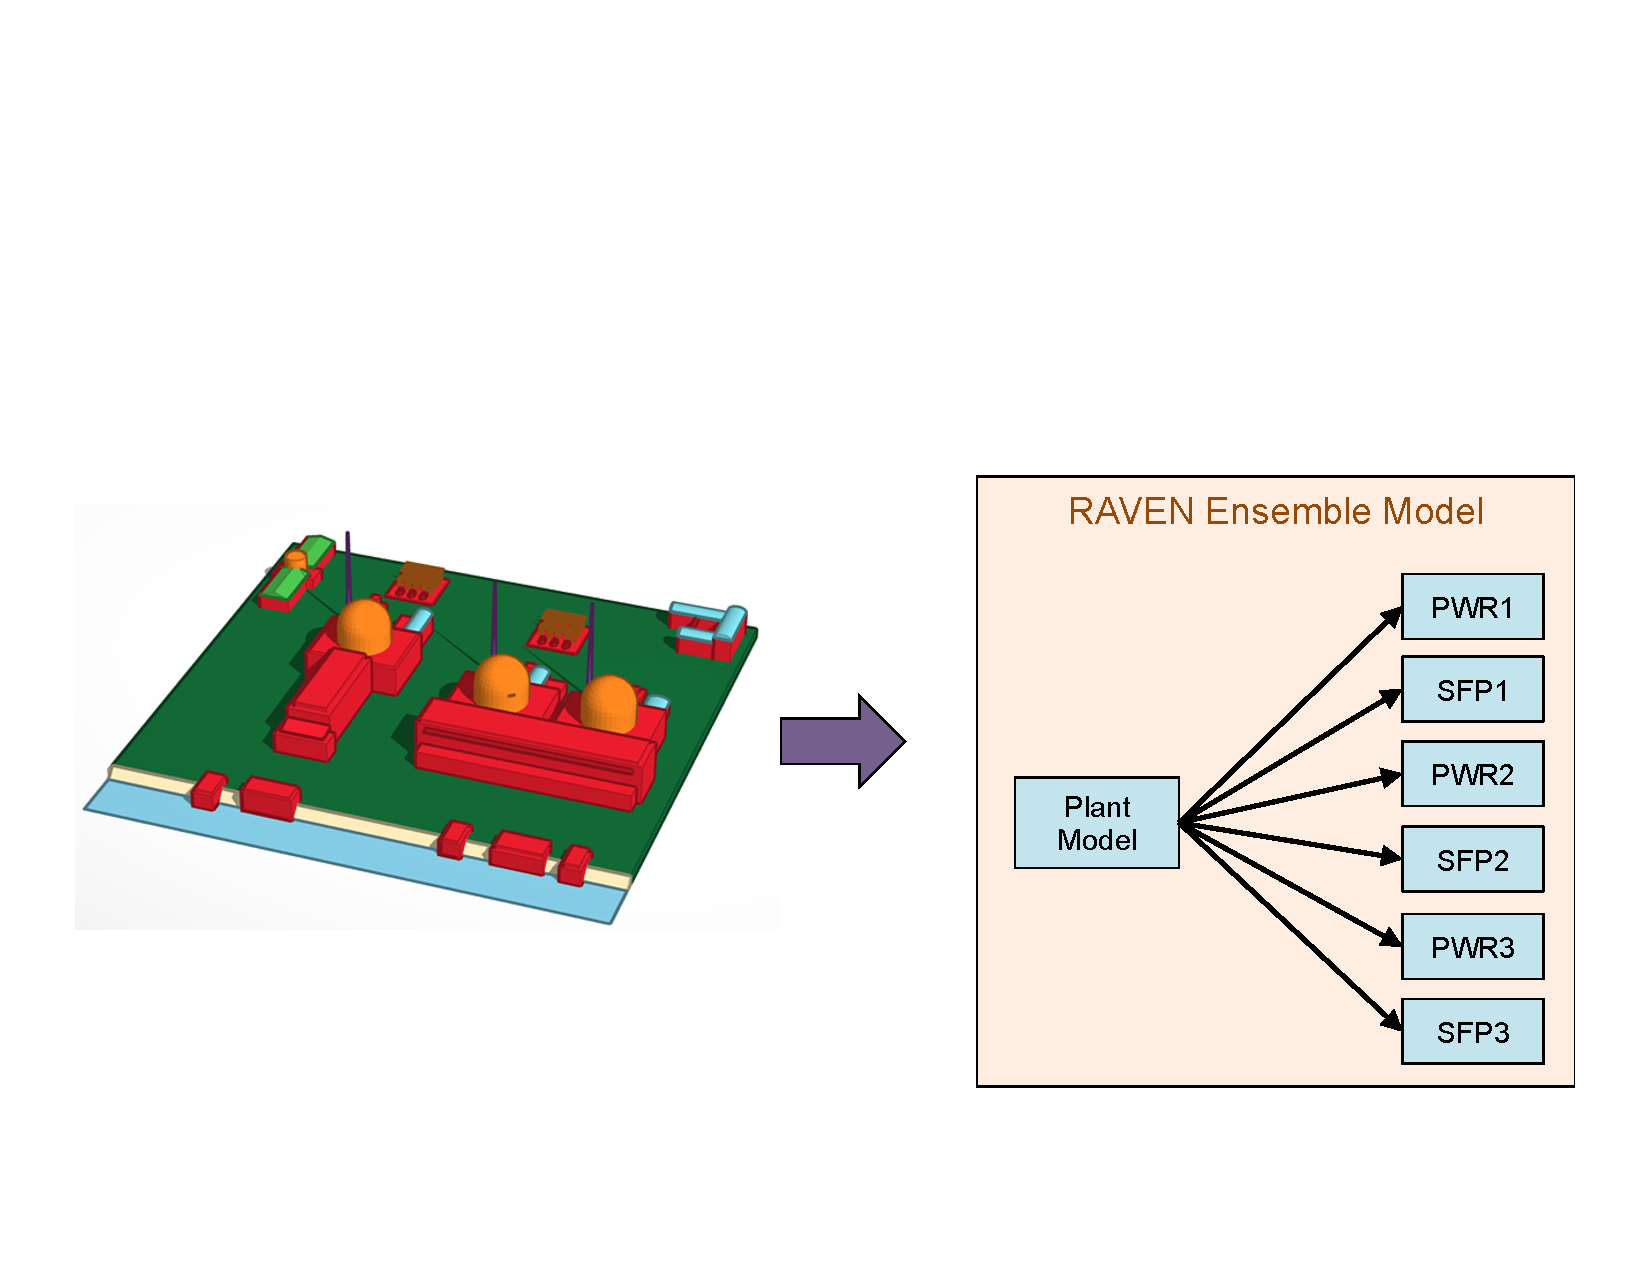
\includegraphics[scale=0.5]{ensembleModel.pdf}
    \caption{RAVEN ensemble model for the considered test case}
    \label{fig:ensembleModel}
\end{figure}

\subsection{System Models}
[CARLO]
\subsubsection{PWR1 and PWR3}

\subsubsection{PWR2}

\subsubsection{SFPs}

\subsubsection{Human models}
[RON]

\subsection{Plant Model}
The plant model has been coded as a Python script and interfaced with RAVEN as an external model. Its
main purpose is to determine timing and sequencing of events for all six system models (i.e., PWRs and 
SFPs) given the sampled values of the stochastic parameters.

\subsection{Plant Stochastic Modeling}

We have identified 